% State of the art, nåværende teknologi og implementasjoner
\section{Current state of XQuery parsers}

There has been much interest and research in XML query languages in recent
years due to the vast amount of information stored in XML documents and the
previously complicated interfaces for retrieving information from these documents.

However these query languages have focused on structural querying and not
content querying with possibilities of full-text matching, for example using
linguistics (such as stemming and thesaurus).

The XQuery language has been extended with full-text capabilities (as described
in section \ref{sect:theory:xquery}), and relevant to this project is a
collection of both full-text enabled XQuery parsers as well as regular XQuery
parsers. This section will outline some of the most interesting implementations.

\subsection{Full-text implementations}
\subsubsection{Quark / TexQuery}
\begin{figure}[!h]
  \centering
    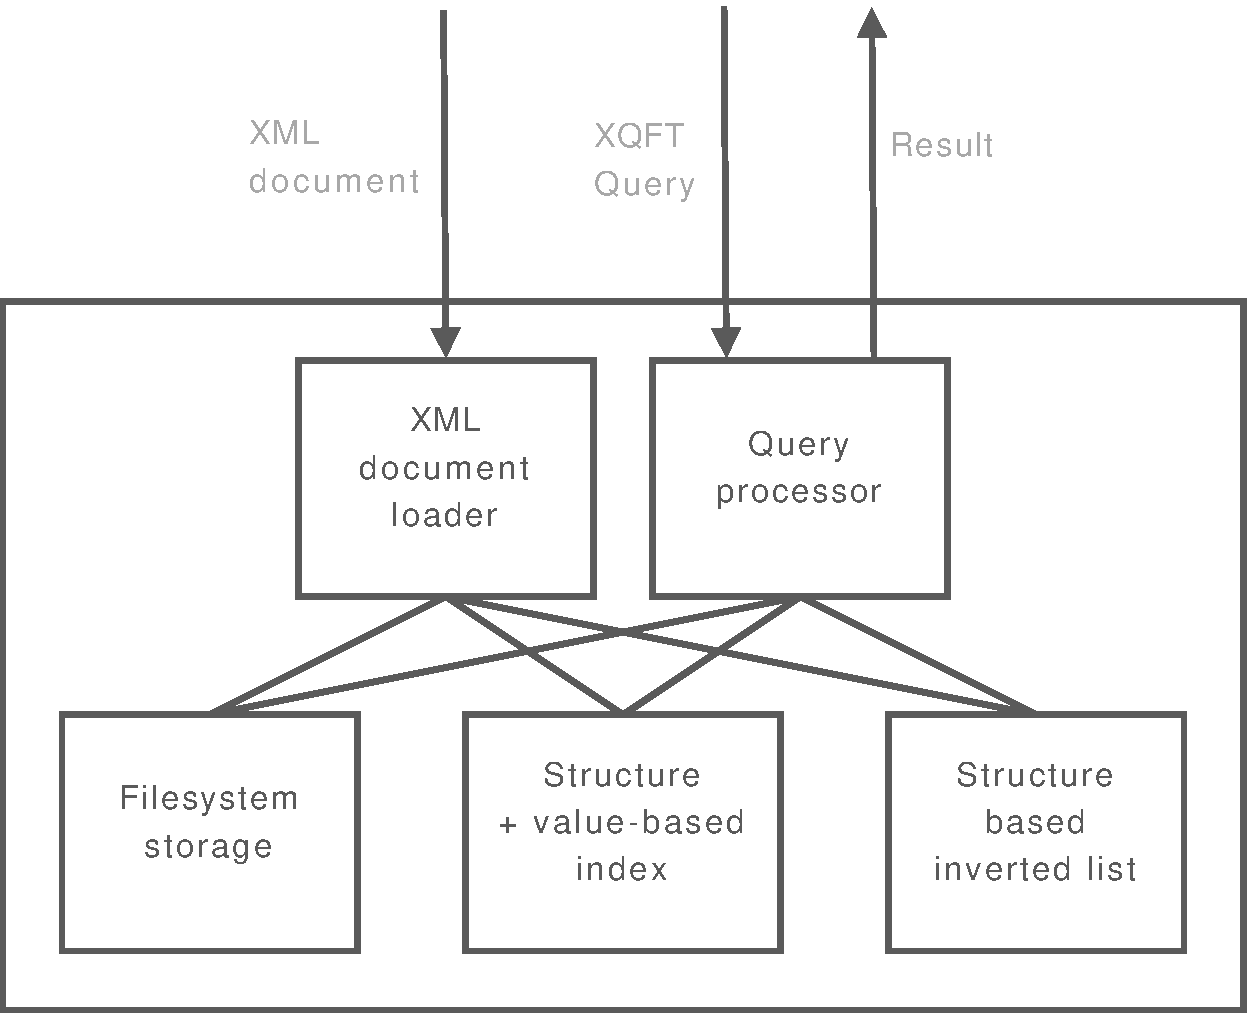
\includegraphics[width=0.6\textwidth]{diagrams/quark_arch}
  \caption{Quark architecture, based on architecture described in
  \cite{quark_efficientxquery}}
\end{figure}

Quark is an experimental full-text search engine capable of indexing and
querying XML documents, and it uses the TexQuery query language (see below). 
Quark was developed as a research project at Cornell University by Jayavel 
Shanmugasundaram and his associates.

\begin{figure}[!h]
  \centering
    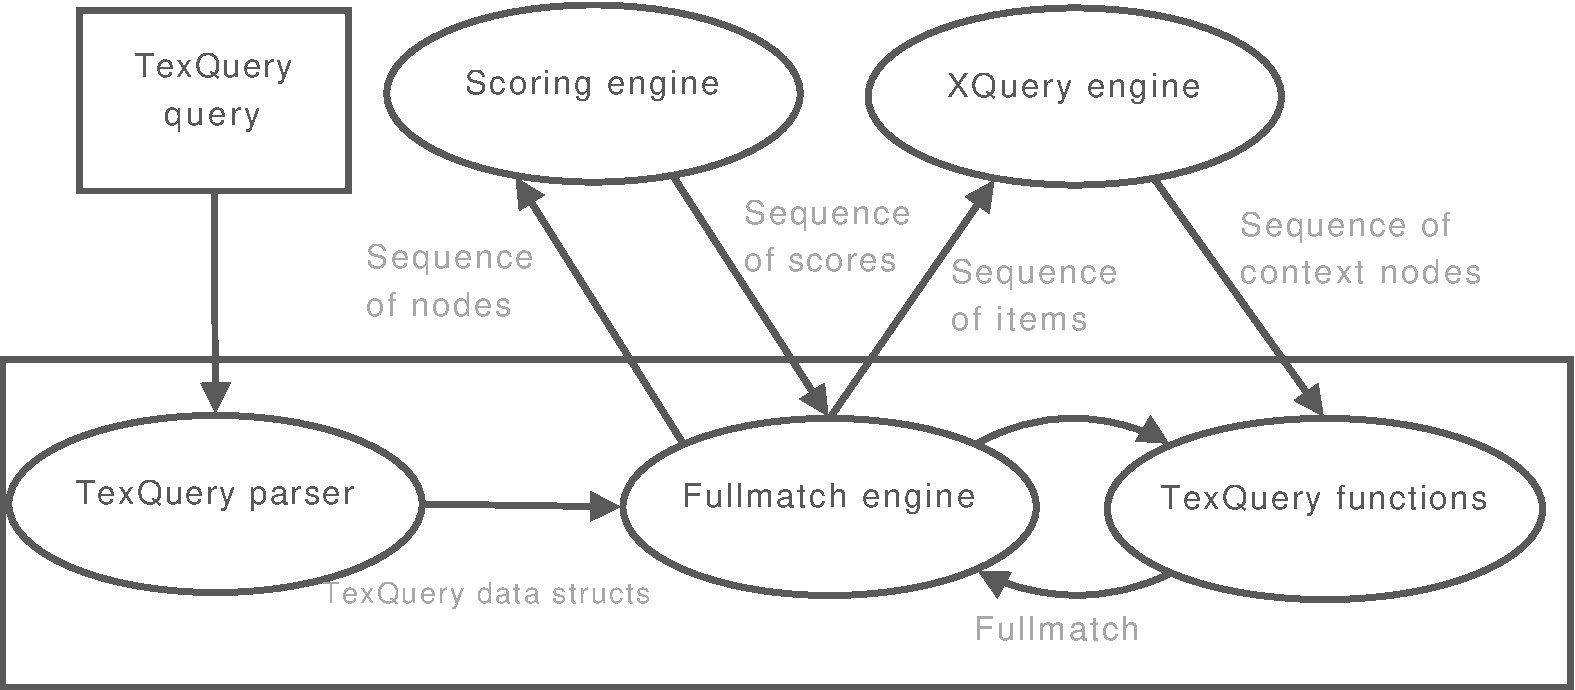
\includegraphics[width=0.7\textwidth]{diagrams/texquery_arch}
  \caption{TexQuery architecture, based on architecture described in \cite{texquery_fulltextsearch}}
\end{figure}

TexQuery is a query language extending upon Xquery with added full-text search 
capabilities. These extensions do not necessarily conform to the W3C
recommendation, however TexQuery is an early precursor to the current W3C 
recommendation \cite{TEXQ00}, in whose development Shanmugasundaram actively 
participates. The source code for this project is available at the Quark Project
website\cite{quarkproject}.

\subsubsection{Galatex}
\begin{figure}[!h]
  \centering
    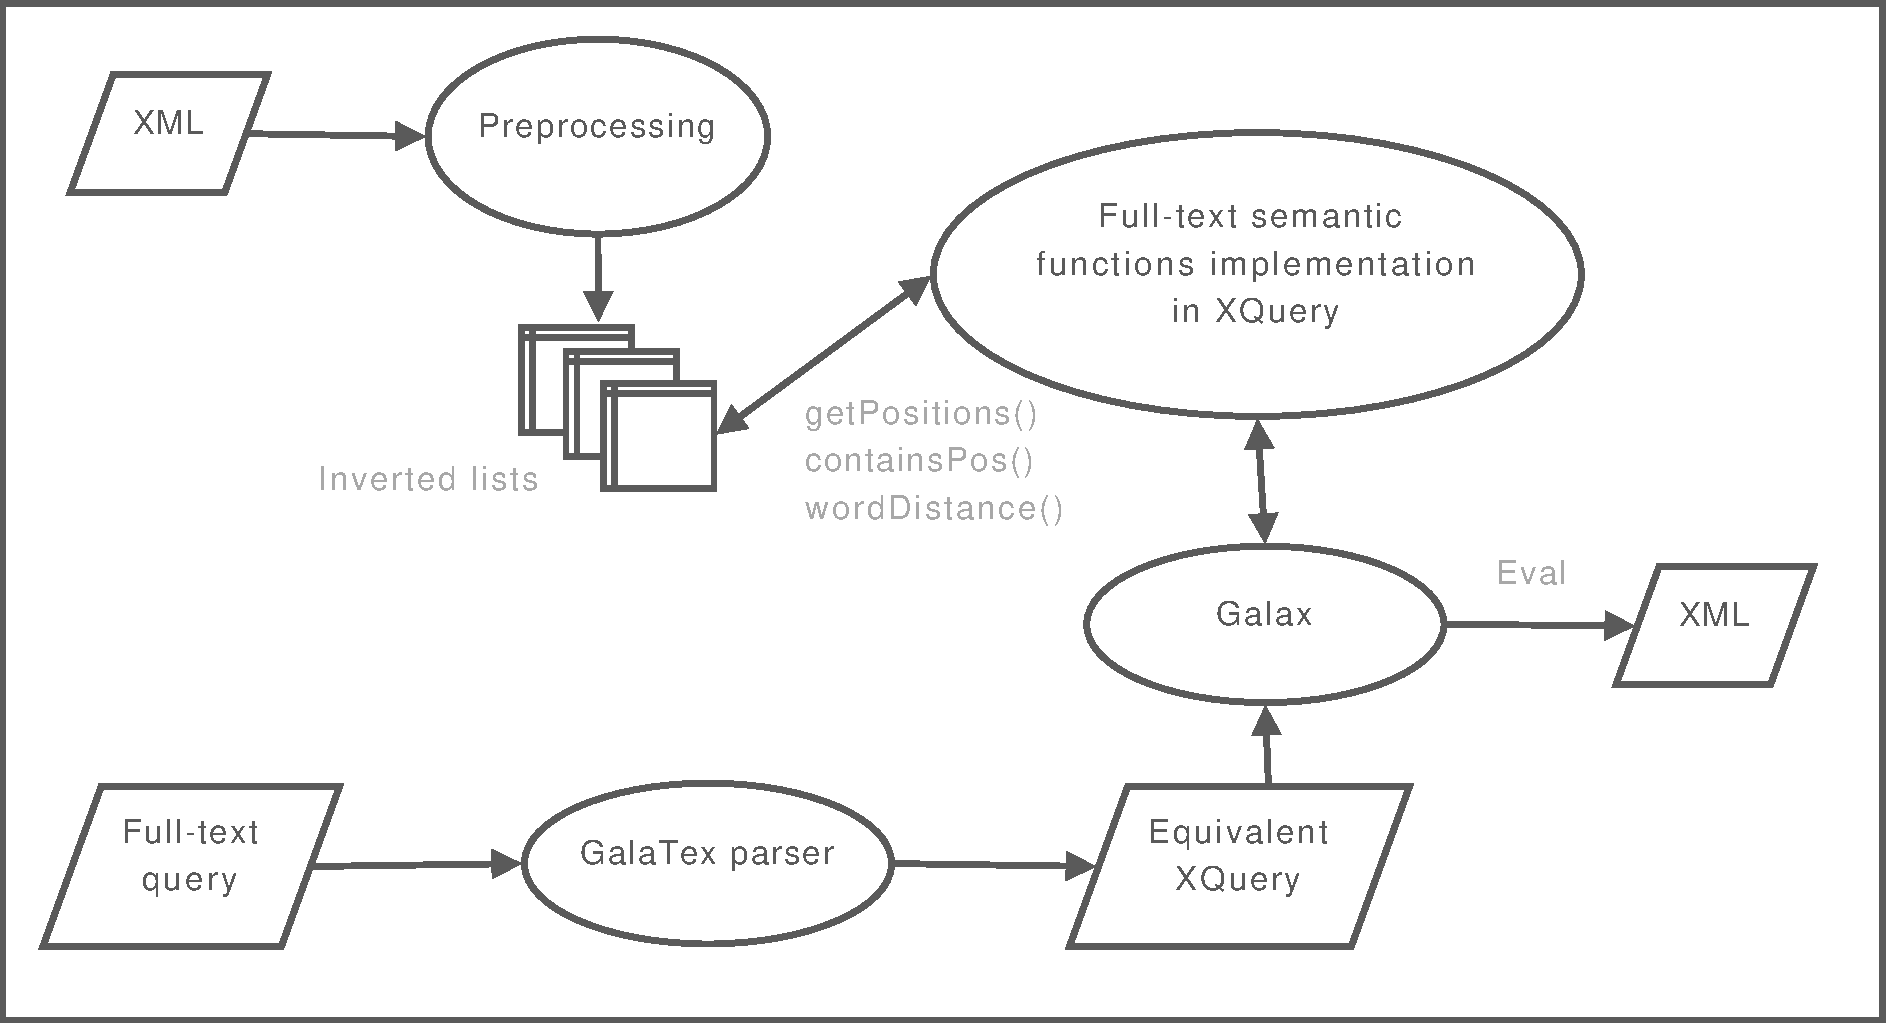
\includegraphics[width=1\textwidth]{diagrams/galatex_arch}
  \caption{Galatex architecture, based on architecture described on the GalaTex
  website\cite{galatex}}
\end{figure}

GalaTex is a complete implementation of the Xquery 1.0 and Xpath 2.0
specifications with full-text extensions. GalaTex is an extension of Galax,
which is a generic Xquery engine. The XQFT query is parsed and converted to an
equivalent XQuery query which is passed to the Galax query engine. The GalaTex
source code is licensed under a non-commercial license developed to AT\&{}T 
\footnote{http://www.galaxquery.com/galatex/LICENSE} and is available at the
GalaTex website \cite{galatex}.

\subsubsection{eXist}
\label{sect:stateOfTheArt:eXist}

\begin{figure}[!h]
  \centering
    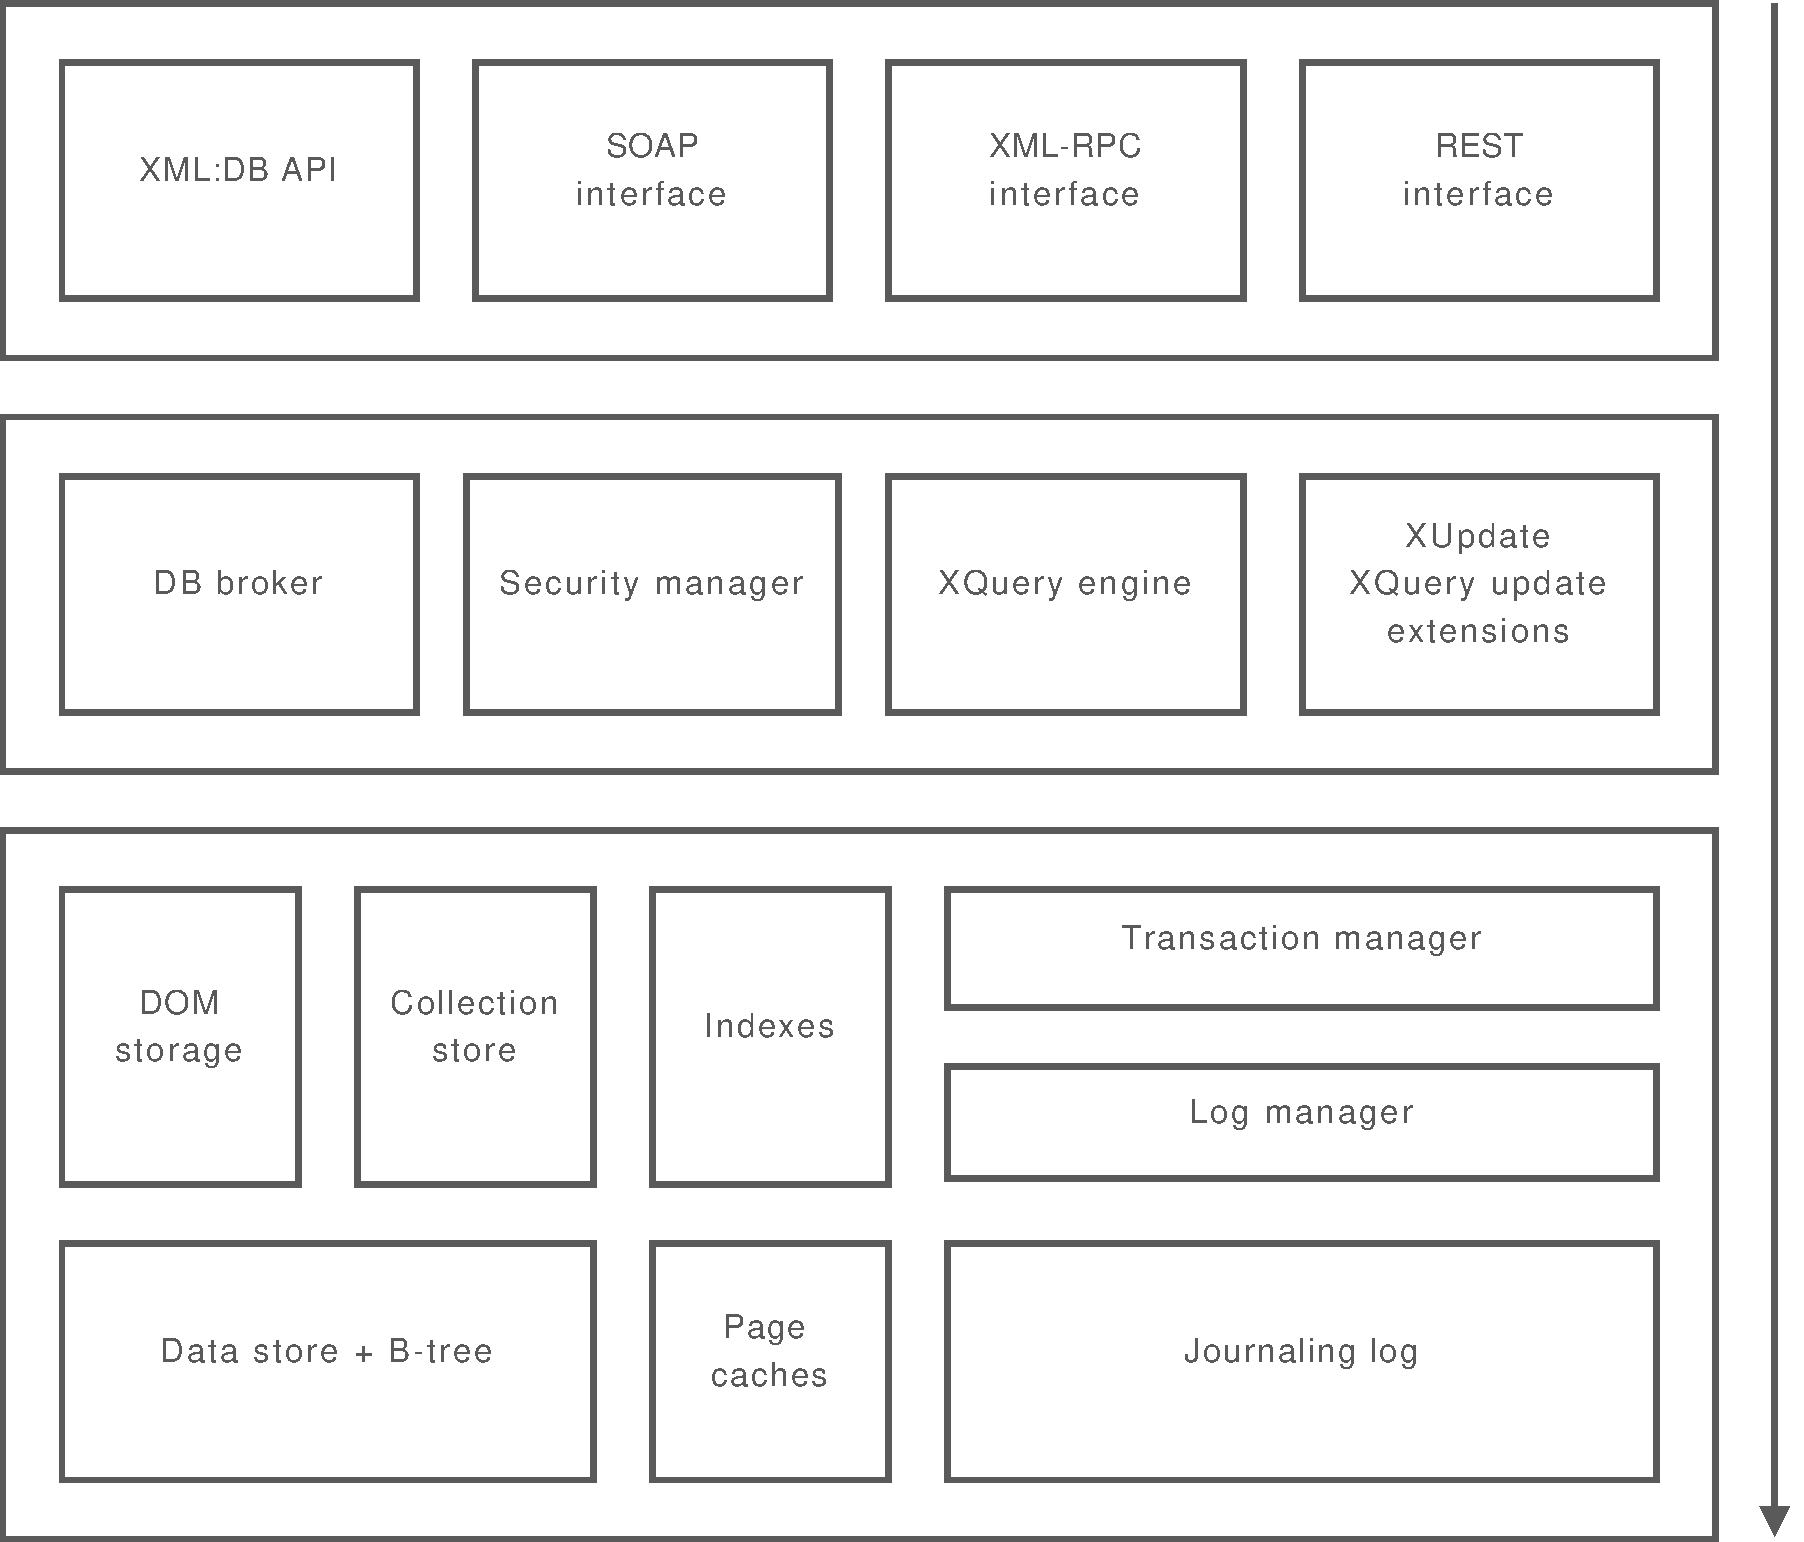
\includegraphics[width=0.9\textwidth]{diagrams/exist_arch}
  \caption[eXist architecture]{eXist architecture, based on architecture sketch
  from \cite{exist_indexdriven}}
\end{figure}

eXist is an open source native XML database system, with an advanced XQuery
query engine with support for full-text extensions. eXist has an approach to
XQuery processing coined as ``Index-driven XQuery processing''
\cite{exist_idx_drv_query}.

eXist is an especially interesting implementation, not only because of its
full-text capabilities, but also because the XQuery parser is generated using
ANTLR, the parser generator that would later be chosen for this particular
project (see section \ref{sect:method:alternatives}).

The full-text capabilities in eXist are however limited. They are not based on
the W3C specification, but rather on a very simplified custom set of operators
and utility functions. The eXist documentation\cite{exist_doc} describes the
following two operators:

\begin{itemize}
  \item \emph{<node-set> \&= 'keywords'}: This operator selects nodes from the
  left-hand argument containing all of the keywords in the right-hand argument 
  in any order
  \item \emph{<node-set> |= 'keywords'}: This operator selects nodes from the
  left-hand argument containing any of the keywords in the right-hand argument
\end{itemize}

Additionally, the following functions are available:
\begin{itemize}
  \item \emph{near(<node-set>, 'keywords' [, max-distance])}: Measures the 
  distance between search terms by counting the number of words between 
  them.
  \item \emph{match-all(node-set, 'regexp' [, 'regexp' \ldots])}: returns
  nodes from the node-set that matches the all of the given regular expressions 
  \item \emph{match-any(node-set, 'regexp' [, 'regexp' \ldots])}: returns nodes
  from the node-set that matches any which one of the regular expressions
\end{itemize}

In it's simplicity, these are powerful extensions to vanilla XQuery, however
linguistics such as stemming, thesaurus and diacritics are not taken into
consideration.

The source code and several other resources are available at the eXist
website\cite{existweb}. 

\subsection{Implementations sans full-text extensions}
There are a wealth of XQuery implementations without full-text
extensions available, in this section we will list some implementations of
particular interest to this project.
\subsubsection{Saxon}
Saxon is an open source XSLT and XQuery processor. It is being actively
developed by Michael Kay, and is dual-licensed under the Mozilla Public License
(MPL). Saxon is optionally available under a closed commercial license.

Saxon conforms to the XSLT 2.0, XQuery 1.0 and XPath 2.0 recommendations
by the W3C as of 23rd of january, 2007. 

At the time of writing, Saxon is the only implementation conforming 100\% to
the W3C test suite\cite{w3ctestresults}. The same test suite was used in this
project as a benchmark of conformance, see section \ref{sect:tests:manual}.

\subsubsection{Pathfinder}
\label{sect:soa:pathfinder}
\begin{figure}[!h]
  \centering
    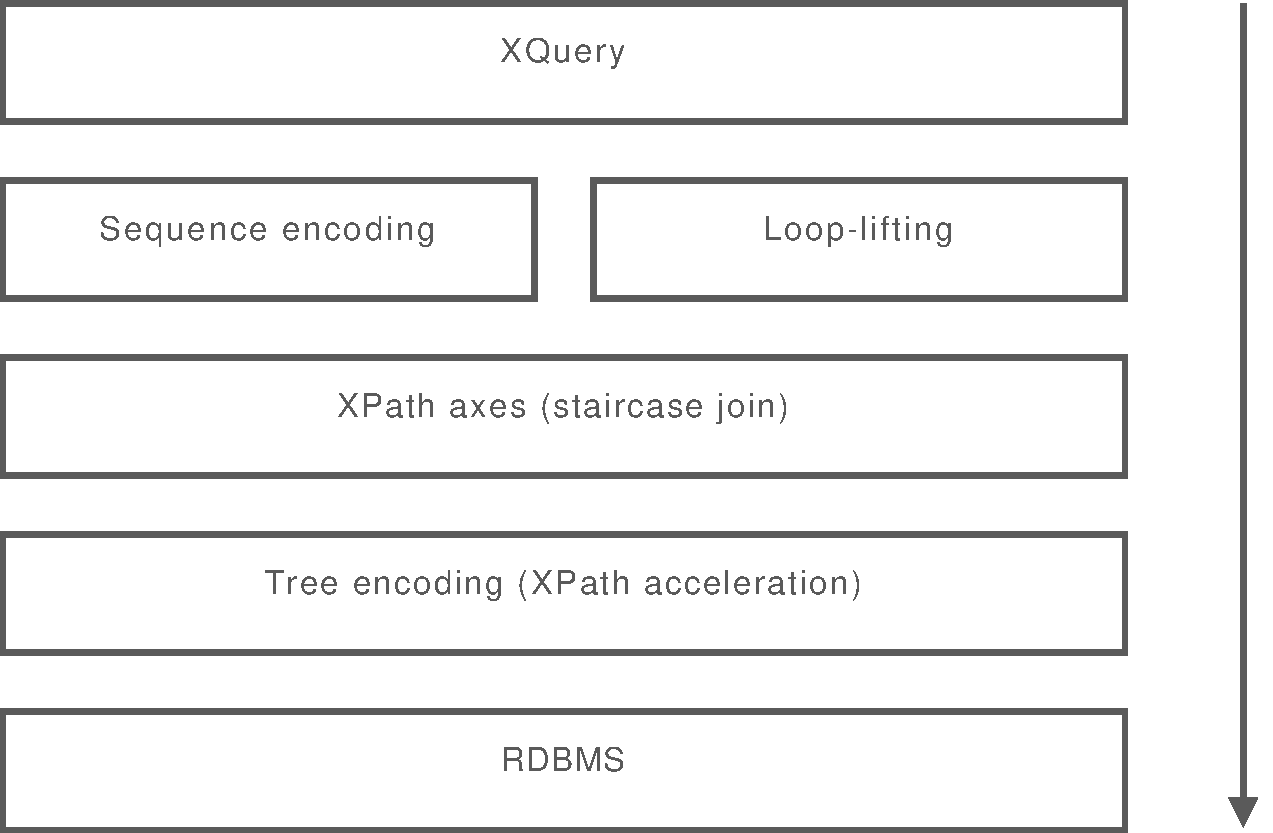
\includegraphics[width=0.6\textwidth]{diagrams/pathfinder_arch}
  \caption{Pathfinder architecture / development stack}
\end{figure}

The Pathfinder project is an XQuery parser running on top of relational
database systems, namely MonetDB. The goal of the Pathfinder project is to
investigate how relational database technology can be utilized to create a
scalable and efficient XQuery implementation. However, the Pathfinder project
has, at the current time of writing, no support for full text extensions. A
future version of Pathfinder is planned to be capable of emitting SQL code
generated from the XQuery parse tree. This illustrates the Pathfinder systems
capabilities of interoperating with relational database systems.

Pathfinder is written in C, and the XQuery parser is a generated using standard
Flex and Bison compiler generator tools.

Pathfinder is and has been a subject of extensive research on coupling XQuery
frontends with relational databases, and a number of papers have been written 
on various areas of interest in the context of Pathfinder, such as compilation
techniques for relational targets\cite{pathfinder_comptech} and loop-lifted
staircase joins\cite{pathfinder_staircase}.
